%%%%%%%%%%%%%%%%%%%%%%%%%%%%%%%%%%%%%%%%%%%%%%%%%%%%%%%%%%%%%%%%%%%%%%%
%
%   Professional Project Report Template
%   Updated by Gemini
%
%%%%%%%%%%%%%%%%%%%%%%%%%%%%%%%%%%%%%%%%%%%%%%%%%%%%%%%%%%%%%%%%%%%%%%%

\documentclass[12pt, a4paper]{report}

% --- CORE PACKAGES ---
\usepackage[a4paper, margin=1in]{geometry} % Page layout and margins
\usepackage{graphicx}                     % For including images
\usepackage{times}                        % Use Times font for a classic look
\usepackage{amsmath, amssymb} 
\usepackage{parskip}
\usepackage[english]{babel}
\usepackage{microtype}

% Teach LaTeX how to hyphenate your specific long words
\hyphenation{stand-alone frame-work-less non-func-tion-al high-fi-del-i-ty}

% --- HYPERLINKS & REFERENCING ---
\usepackage{hyperref}                     % For clickable links and references in the PDF
\usepackage{tabularx}   % For tables that automatically fit the page width
\usepackage{booktabs}   % For professional-looking horizontal lines in tables

\hypersetup{
    colorlinks=true,
    linkcolor=black,    % Color for internal links (e.g., ToC)
    citecolor=black,    % Color for bibliography citations
    urlcolor=black,      % Color for external URLs
    pdftitle={Project Report: RESTful Schema-Aware Data Integration API},
    pdfauthor={Dijith Dinesh, et al.},
    pdfpagemode=FullScreen,
}

% --- HEADER, FOOTER & STYLING ---
\usepackage{fancyhdr}                     % For custom headers and footers
\usepackage{sectsty}                      % To style section and chapter headings

% --- TABLE OF CONTENTS & LISTS ---
\usepackage[toc,page]{appendix}           % For appendices
\usepackage{tocbibind}                    % Adds ToC, LoF, LoT, Bibliography to the ToC

% --- OTHER UTILITIES ---
\usepackage{listings}                     % For formatting code snippets
\usepackage{tabularx}                     % For tables with adjustable column widths

% --- CUSTOM STYLING COMMANDS ---

% Center unnumbered chapters (e.g., Abstract, Acknowledgements)
\chapterfont{\centering}

% Setup for Headers and Footers
\pagestyle{fancy}
\fancyhf{} % Clear all existing header and footer fields
\fancyhead[L]{RESTful Data Integration API}
\fancyhead[R]{\nouppercase{\leftmark}} % Chapter title on the right
\fancyfoot[C]{\thepage}
\renewcommand{\headrulewidth}{0.4pt}
\renewcommand{\footrulewidth}{0.4pt}

% --- DOCUMENT START ---
\begin{document}
\renewcommand{\bibname}{References} % <--- ADD THIS LINE

% --- FRONT MATTER (Title Page, Certificate, etc.) ---
% Pages here will not have headers/footers and will be numbered with Roman numerals later

\begin{titlepage}
    \centering
    \pagestyle{empty} % No header/footer on the title page
    
    \vspace*{1cm}
    
    {\Huge \bfseries RESTful Schema-Aware Data Integration \& Transformation API}
    
    \vspace{0.2cm}
    
    {\large \textbf{PBCST304 Project Report}}
    
    \vfill % Pushes content down
    
    {\large \itshape Submitted by:}
    
    \vspace{1cm}
    
    % Using tabular for a clean, aligned layout of names and IDs
    
    \begin{tabularx}{0.9\textwidth}{X r}
        \bfseries Aaron Paul & \bfseries MDL24CSBS002 \\
        \bfseries Athuljith S & \bfseries MDL24CSBS021 \\
        \bfseries Dijith Dinesh & \bfseries MDL24CSBS023 \\
        \bfseries Peter Joe Menachery & \bfseries MDL24CSBS048 \\
        \bfseries Pranav Manoj & \bfseries MDL24CSBS049 \\
    \end{tabularx}
    
   
    \vfill % Fills the remaining space, pushing the logo and college name down
    
    \includegraphics[width=0.1\textwidth]{college.png}
    
    \vspace{0.5cm}
    
    {\Large \bfseries Department of Computer Engineering} \\
    {\large \bfseries Govt. Model Engineering College, Thrikkakara} \\
    {\large Ernakulam, Kochi 682021} \\
    {\large \href{https://www.mec.ac.in}{https://www.mec.ac.in}} \\
    
    \vspace{1.5cm}
    
    {\large October 2025}
     \vspace{5cm}
    
\end{titlepage}

\newpage

% --- CERTIFICATE ---
\pagestyle{empty} % No header/footer on this page

\begin{center}
    {\Large\bfseries Model Engineering College, Thrikkakara} \\
    {\large\bfseries Department of Computer Engineering} \\
     \vspace{0.6cm}
     \includegraphics[width=0.15\textwidth]{college.png} \\
    \vspace{0.6cm}
    {\Huge\bfseries CERTIFICATE} \\
    \vspace{1cm}
\end{center}

\noindent
This is to certify that the project report entitled:
    \large{\bfseries{ “RESTful Schema-Aware Data Integration \& Transformation API”}}
\noindent
is a bonafide record of the work carried out by
\begin{center}
    \begin{tabularx}{0.9\textwidth}{X r}
        \bfseries Aaron Paul & MDL24CSBS002 \\
        \bfseries Athuljith S & MDL24CSBS021 \\
        \bfseries Dijith Dinesh & MDL24CSBS023 \\
        \bfseries Peter Joe Menachery & MDL24CSBS048 \\
        \bfseries Pranav Manoj & MDL24CSBS049 \\
    \end{tabularx}\\
    \textbf{Third semester B.Tech  Computer Science \& Engineering \& Business Systems}
\end{center}

\noindent
students, in partial fulfillment of the requirements for the course \textbf{PBCST304: Object Oriented Programming} for the award of the degree of Bachelor of Technology from \textbf{APJ Abdul Kalam Technological University}.

\vfill % Pushes the signatures to the bottom

\begin{tabular}{p{0.45\textwidth} p{0.45\textwidth}}
    \hrulefill & \hfill \hrulefill \\
    \textbf{Raheena Salihin} & \hfill \textbf{Dr. Binu V P} \\
    \textit{Project Guide} & \hfill \textit{Head of the Department} \\
    Assistant Professor & \hfill Associate Professor \\
    Dept. of Computer Engineering & \hfill Dept. of Computer Engineering \\
\end{tabular}
\vspace{3cm}
\begin{flushleft}
    \today \\
   
\end{flushleft}

\newpage

% --- ACKNOWLEDGEMENTS ---
\chapter*{Acknowledgements}
\thispagestyle{fancy} % Use fancy style, but it will be mostly empty due to \chapter*

We wish to extend our profound gratitude to the individuals whose guidance and support were instrumental in the successful completion of this project.

Our deepest appreciation is reserved for our project guide, \textit{Raheena Salihin}. Her technical acumen and rigorous feedback were pivotal in transforming our initial concept into a robust and functional application. Her mentorship consistently challenged us to think critically, adhere to the highest standards of software engineering, and navigate the complexities of system architecture.

We are also grateful to our Head of Department, \textit{Dr. Binu V P}, and the entire faculty of the Department of Computer Engineering for fostering an academic environment that encourages innovation and for providing the administrative support essential for our work.

Finally, we thank our peers for their collaborative spirit and our families for their enduring patience and support throughout this endeavor.

\vspace{3cm}
\begin{flushright}
    \textbf{Aaron Paul} MDL24CSBS002 \\
    \textbf{Athuljith S} MDL24CSBS021 \\
    \textbf{Dijith Dinesh} MDL24CSBS023 \\
    \textbf{Peter Joe Menachery} MDL24CSBS048 \\
    \textbf{Pranav Manoj} MDL24CSBS049
\end{flushright}

\newpage

% --- ABSTRACT ---
\chapter*{Abstract}
In modern software development, client applications are often tightly coupled to the database schema of backend services, leading to brittle and difficult-to-maintain systems. Any change in the backend schema can cause cascading failures, necessitating costly update cycles for all client applications. This project addresses this critical issue by designing and implementing a \textbf{RESTful Schema-Aware Data Integration and Transformation API}.

This system acts as an intelligent, universal data gateway that completely decouples client applications from the physical database. It provides a robust abstraction layer that allows clients to fetch, filter, sort, and transform data using a simple, intuitive URL-based query language, abstracting away the complexities of SQL. The API supports on-the-fly data transformation into multiple formats (JSON, CSV, XML) and dynamic field renaming through a powerful view-management system.

Built from the ground up in Java without external frameworks, the project is a case study in applying core Object-Oriented principles—Encapsulation, Inheritance, Polymorphism, and Abstraction—to build a modular, maintainable, and secure backend service. The system enforces security through a role-based access control (RBAC) mechanism using API keys, providing a centralized and managed access point to data. The final product is a lightweight, powerful, and flexible tool for any developer needing to expose data securely and efficiently.

\newpage

% --- TABLE OF CONTENTS, LIST OF FIGURES, LIST OF TABLES ---
% These will be numbered with Roman numerals
\pagenumbering{roman}
\pagestyle{fancy} % Re-apply fancy style for ToC pages

\tableofcontents
\newpage

\listoffigures
\newpage

\listoftables % This will be empty if you have no tables, but it's good practice to include
\newpage

% --- MAIN MATTER (Actual Report Chapters) ---
% Switch to Arabic numbering and restart at 1
\cleardoublepage
\pagenumbering{arabic}

%%%%%%%%%%%%%%%%%%%%%%%%%%%%%%%%%%%%%%%%%%%%%%%%%%%%%%%%%%%%%%%%%%%%%%%
% --- CHAPTER 1: INTRODUCTION ---
%%%%%%%%%%%%%%%%%%%%%%%%%%%%%%%%%%%%%%%%%%%%%%%%%%%%%%%%%%%%%%%%%%%%%%%
\chapter{Introduction}
\section{Proposed Project}
This document outlines the design, architecture, and implementation of the RESTful Schema-Aware Data Integration and Transformation API. The project's core mission is to solve a pervasive problem in software architecture: the tight coupling between client applications and backend data sources. By providing a flexible and intelligent middleware, this project aims to streamline development, enhance system resilience, and improve data security.

\subsection{Problem Statement}
In contemporary application development, client-side software (such as web frontends, mobile apps, or other backend services) is frequently designed to consume data directly from a backend database. This direct or near-direct interaction leads to several significant problems:
\begin{itemize}
    \item \textbf{Brittleness and High Maintenance Overhead:} Client applications often contain logic that is explicitly tied to the database schema. If a database administrator renames a column (e.g., from \lstinline!user_email! to \lstinline!email_address!), every client application that references the old column name will break. This necessitates a coordinated, and often costly, update and redeployment of all dependent applications.
    \item \textbf{Developer Inefficiency:} Client-side developers are forced to write repetitive boilerplate code to fetch, parse, and transform data into the specific format required by their application's views or models. This introduces redundancy and distracts from the core task of building user-facing features.
    \item \textbf{Lack of a Single Source of Truth:} When data logic is scattered across multiple client applications, there is no centralized point of control for data access rules, validation, or transformation. This leads to inconsistencies and makes the system difficult to manage.
    \item \textbf{Security Risks:} Exposing database structures, even indirectly, can create security vulnerabilities. Furthermore, managing fine-grained access control across numerous disparate clients is a complex and error-prone task.
\end{itemize}
These issues collectively lead to systems that are difficult to evolve, expensive to maintain, and insecure.

\subsection{Proposed Solution}
To address the challenges outlined above, we propose the development of a standalone, universal API server that acts as an abstraction layer between clients and the physical database. This \textbf{RESTful Schema-Aware Data Gateway} provides a comprehensive solution:
\begin{itemize}
    \item \textbf{Decoupling through Abstraction:} The API completely decouples clients from the database. Clients interact with a stable, well-defined RESTful interface, while the API server is responsible for translating these requests into the appropriate database queries. If the database schema changes, only the API's internal mapping needs to be updated, leaving all client applications unaffected.
  \item \textbf{Brittleness and High Maintenance Overhead:} Client applications often contain logic that is explicitly tied to the database schema. If a database administrator renames a column (e.g., from \lstinline!user_email! to \lstinline!email_address!), every client application that references the old column name will break. This necessitates a coordinated, and often costly, update and redeployment of all dependent applications.
    \item \textbf{On-the-Fly Data Transformation:} The API can deliver data in a variety of formats (JSON, CSV, XML, etc.) based on a simple URL parameter (`?format=csv`). It also features a powerful "view" system that allows for dynamic renaming of data fields, enabling clients to receive data in the exact structure they require without any backend code changes.
    \item \textbf{Centralized Security and Control:} The API enforces a Role-Based Access Control (RBAC) model using API keys. Permissions (read-only, write, admin) are managed centrally, providing a single, secure, and auditable point of access to the data.
\end{itemize}
This approach establishes a single centralized source of truth for data access, significantly reduces the client-side development effort, and creates a more secure, resilient, and maintainable system architecture.

%%%%%%%%%%%%%%%%%%%%%%%%%%%%%%%%%%%%%%%%%%%%%%%%%%%%%%%%%%%%%%%%%%%%%%%
% --- CHAPTER 2: SOFTWARE REQUIREMENT SPECIFICATION (SRS) ---
%%%%%%%%%%%%%%%%%%%%%%%%%%%%%%%%%%%%%%%%%%%%%%%%%%%%%%%%%%%%%%%%%%%%%%%
\chapter{Software Requirement Specification (SRS)}

\section{Introduction}
This chapter provides a detailed specification of the requirements for the RESTful Schema-Aware Data Integration API. It outlines the functional and non-functional requirements, constraints, and system attributes, serving as the primary reference for the design, development, and testing phases of the project.

\subsection{Purpose}
The purpose of this Software Requirement Specification (SRS) document is to provide a clear, comprehensive, and unambiguous description of the system's intended behavior and capabilities. It aims to:
\begin{itemize}
    \item Establish a formal agreement between the development team and stakeholders on what the software will and will not do.
    \item Serve as the foundational blueprint for all subsequent project activities, including architectural design, implementation, and quality assurance.
    \item Provide a baseline for evaluating and verifying the final product against the initial requirements.
\end{itemize}

\subsection{Intended Audience}
This document is intended for a wide range of stakeholders, including:
\begin{itemize}
    \item \textbf{Project Developers:} To understand the system's requirements and constraints, guiding their implementation efforts.
    \item \textbf{System Architects:} To design a robust and scalable architecture that meets the specified requirements.
    \item \textbf{Testers and QA Engineers:} To create test plans and test cases that ensure the system behaves as expected.
    \item \textbf{Project Managers:} To manage the project scope and track progress against the defined requirements.
    \item \textbf{End-Users (Client Developers):} To understand the capabilities and limitations of the API they will be consuming.
\end{itemize}

\subsection{Project Scope}
The project scope is to develop a standalone, general-purpose RESTful API server that can be placed in front of any relational database to provide a flexible and secure data access layer.

\textbf{In Scope:}
\begin{itemize}
    \item Development of a runnable Java application that starts a lightweight HTTP server.
    \item Implementation of API endpoints for data querying (CRUD operations), schema discovery, and view management.
    \item A dynamic URL parser that can translate query parameters into secure SQL.
    \item A modular data export system for transforming data into multiple formats (JSON, CSV, XML, etc.).
    \item A role-based access control (RBAC) system based on API keys stored in the database.
    \item An administrative endpoint for executing a limited set of secure DDL commands.
\end{itemize}

\textbf{Out of Scope:}
\begin{itemize}
    \item Development of any client-side applications (web UIs, mobile apps). The project focuses solely on the backend API server.
    \item User authentication systems (e.g., OAuth, JWT). The API handles authorization via its own keys, but assumes user authentication is managed by the client application.
    \item Support for NoSQL databases. The initial design is focused on JDBC-compliant relational databases.
    \item A graphical user interface (GUI) for administering the API. All administration is handled via API endpoints.
\end{itemize}

\section{Overall Description}
\subsection{Product Perspective}
The RESTful API is a self-contained, standalone middleware product. It is not an end-user application but a backend service intended to be used by other software systems. It operates independently of any specific client application or business domain, functioning as a generic and reusable data gateway.

\subsection{Product Functions}
The major functions of the system are summarized below:
\begin{enumerate}
    \item \textbf{Dynamic Data Retrieval:} Allow authorized clients to fetch data from any table using a flexible set of URL parameters for filtering, sorting, pagination, and field selection.
    \item \textbf{On-the-Fly Data Transformation:} Convert raw database results into various client-requested formats (e.g., JSON, CSV) and restructure the data's field names using predefined or ad-hoc views.
    \item \textbf{Secure Data Modification:} Provide secure endpoints for creating, updating, and deleting records, subject to authorization rules.
    \item \textbf{Schema Discovery:} Enable clients to programmatically query the schema of database tables, including column names and data types.
    \item \textbf{Centralized Security:} Authenticate all requests via API keys and authorize actions based on the roles (read, write, admin) associated with each key.
    \item \textbf{Administrative Control:} Offer a secure endpoint for administrators to perform basic database management tasks.
\end{enumerate}

\subsection{User Classes and Characteristics}
\begin{description}
    \item[Client Developer:] The primary user of the API. This user is a software developer building a client application. They are expected to have a good understanding of RESTful principles and HTTP. They require a well-documented, intuitive, and powerful API to accelerate their development process.
    \item[System Administrator:] This user is responsible for deploying, configuring, and maintaining the API server. They have a technical background in systems administration and database management. They require secure access to administrative functions to manage the database schema and API keys.
\end{description}

\subsection{Operating Environment}
The API server is designed to be platform-independent and will operate in the following environment:
\begin{itemize}
    \item \textbf{Operating System:} Any modern 64-bit operating system that can run a Java Virtual Machine (JVM), including Windows, Linux, and macOS.
    \item \textbf{Runtime Environment:} Java Development Kit (JDK) 11 or newer.
    \item \textbf{Database:} The system will interface with any JDBC-compliant relational database. It is developed and tested with SQLite for portability but is designed to be easily configurable for databases like PostgreSQL, MySQL, etc.
\end{itemize}

\subsection{Design and Implementation Constraints}
\begin{itemize}
    \item The system must be implemented in Java without the use of major external frameworks like Spring or Jakarta EE to ensure a lightweight footprint and focus on core OOP principles.
    \item All database queries generated from user input must be parameterized to prevent SQL injection vulnerabilities. Direct string concatenation of user input into SQL queries is strictly forbidden.
    \item The final deliverable must be a self-contained, runnable application (e.g., a JAR file) that can be easily deployed and started from the command line.
    \item The system's internal architecture must be modular and adhere to the principles of high cohesion and loose coupling.
\end{itemize}

\section{Hardware and Software Requirements}
\subsection{Hardware Requirements}
\begin{itemize}
    \item \textbf{CPU:} 2-core x86-64 CPU, 2.0 GHz or faster.
    \item \textbf{RAM:} Minimum of 2 GB RAM. Recommended 4 GB or more for handling a large number of concurrent requests.
    \item \textbf{Storage:} Minimum of 500 MB of free disk space for the application, logs, and a small database.
\end{itemize}

\subsection{Software Requirements}
\begin{itemize}
    \item \textbf{Server OS:} Windows Server 2012+, Ubuntu 18.04+, CentOS 7+, or equivalent.
    \item \textbf{Runtime:} Java SE Development Kit (JDK) 11 or later.
    \item \textbf{Database Engine:} SQLite 3.x (for default operation) or a network-accessible instance of PostgreSQL, MySQL, etc.
    \item \textbf{Testing Client:} A command-line tool capable of making HTTP requests, such as `curl`.
\end{itemize}

\section{Functional Requirements}
This section details the functional requirements of the system, specified by feature.

% --- FR-1 ---
\noindent % Prevents paragraph indentation
\textbf{FR-1: API Key Authentication}
\begin{itemize}
    \item \textbf{FR-1.1:} The system shall require an API key to be sent in the \lstinline|Authorization| HTTP header for all requests to protected endpoints.
    \item \textbf{FR-1.2:} The system shall validate the provided API key against the \lstinline|api_keys| table in the database.
    \item \textbf{FR-1.3:} Requests with missing or invalid API keys shall be rejected with a \lstinline|401 Unauthorized| status.
\end{itemize}

% --- FR-2 ---
\noindent\textbf{FR-2: Dynamic Data Retrieval (GET)}
\begin{itemize}
    \item \textbf{FR-2.1 Filtering (\lstinline|where|):} The system shall allow clients to filter results based on column values using operators such as \lstinline|eq|, \lstinline|neq|, \lstinline|gt|, \lstinline|gte|, \lstinline|lt|, \lstinline|lte|, \lstinline|like|, \lstinline|contains|, and \lstinline|in|.
    \item \textbf{FR-2.2 Sorting (\lstinline|sort|):} The system shall allow clients to sort results by one or more columns in ascending (\lstinline|asc|) or descending (\lstinline|desc|) order.
    \item \textbf{FR-2.3 Pagination (\lstinline|limit|, \lstinline|page|):} The system shall support pagination of results.
    \item \textbf{FR-2.4 Field Selection (\lstinline|fields|):} The system shall allow clients to specify a comma-separated list of columns to be included in the response.
\end{itemize}

% --- FR-3 ---
\noindent\textbf{FR-3: Data Modification (POST, PUT, DELETE)}
\begin{itemize}
    \item \textbf{FR-3.1 Create (\lstinline|POST|):} An authorized client shall be able to create a new record in a table by sending a JSON object in the request body.
    \item \textbf{FR-3.2 Update (\lstinline|PUT|/\lstinline|PATCH|):} An authorized client shall be able to update an existing record by its ID.
    \item \textbf{FR-3.3 Delete (\lstinline|DELETE|):} An authorized client shall be able to delete one or more records that match a \lstinline|where| clause. Mass deletion without a \lstinline|where| clause must be forbidden.
\end{itemize}

% --- FR-4 ---
\noindent\textbf{FR-4: Data Transformation}
\begin{itemize}
    \item \textbf{FR-4.1 Format Export (\lstinline|format|):} The system shall be able to return data in multiple formats, including JSON (default), CSV, XML, HTML, and Markdown, based on the \lstinline|format| URL parameter.
    \item \textbf{FR-4.2 View Management (\lstinline|view|):} The system shall allow users to create, read, and use persistent views that map database column names to client-friendly aliases.
    \item \textbf{FR-4.3 Ad-hoc Renaming (\lstinline|replace|):} The system shall support temporary, one-off renaming of fields in the output using the \lstinline|replace| parameter.
\end{itemize}

% --- FR-5 ---
\noindent\textbf{FR-5: Schema Discovery}
\begin{itemize}
    \item \textbf{FR-5.1:} A client shall be able to retrieve the schema (column names and data types) of any accessible table via the \lstinline|/schema/{tableName}| endpoint.
\end{itemize}
        
% --- FR-6 ---
\noindent\textbf{FR-6: Administrative Functions}
\begin{itemize}
    \item \textbf{FR-6.1:} A client with admin-level privileges shall be able to execute DDL commands (\lstinline|CREATE TABLE|, \lstinline|DROP TABLE|) via the \lstinline|/admin/execute| endpoint.
    \item \textbf{FR-6.2:} The admin endpoint must validate incoming SQL to ensure it is a single, non-malicious command.
\end{itemize}

\section{Non-functional Requirements}

% --- NFR-1 ---
\noindent\textbf{NFR-1: Performance}
\begin{itemize}
    \item \textbf{NFR-1.1 Response Time:} For simple queries on indexed columns, the API should have an average response time of less than 200ms under normal load.
    \item \textbf{NFR-1.2 Concurrency:} The system should be able to handle at least 50 concurrent requests without significant performance degradation.
\end{itemize}

% --- NFR-2 ---
\noindent\textbf{NFR-2: Scalability}
\begin{itemize}
    \item The system's architecture should allow it to scale vertically (by adding more CPU/RAM) and be deployable in a horizontally scaled environment (behind a load balancer).
\end{itemize}

% --- NFR-3 ---
\noindent\textbf{NFR-3: Security}
\begin{itemize}
    \item The system must be protected against SQL injection attacks by exclusively using parameterized queries.
    \item Access to write and admin functionalities must be strictly enforced by the RBAC mechanism.
    \item The system should not expose any sensitive information, such as database credentials or stack traces, in its error responses to the client.
\end{itemize}

% --- NFR-4 ---
\noindent\textbf{NFR-4: Reliability}
\begin{itemize}
    \item The system should be reliable, with an expected uptime of 99.9\%.
    \item The system must handle errors gracefully and return appropriate HTTP status codes and error messages. It should not crash due to invalid user input.
\end{itemize}

% --- NFR-5 ---
\noindent\textbf{NFR-5: Usability (for Developers)}
\begin{itemize}
    \item The API endpoints and URL query parameters must be intuitive, consistent, and easy to use.
    \item Error messages returned by the API should be clear and helpful to a developer trying to debug an issue.
\end{itemize}

% --- NFR-6 ---
\noindent\textbf{NFR-6: Maintainability}
\begin{itemize}
    \item The source code must be well-documented, with comments explaining complex logic.
    \item The project must be structured into logical, modular packages that follow the principles of high cohesion and loose coupling.
\end{itemize}
\clearpage
%%%%%%%%%%%%%%%%%%%%%%%%%%%%%%%%%%%%%%%%%%%%%%%%%%%%%%%%%%%%%%%%%%%%%%%
% --- CHAPTER 3: SYSTEM DESIGN ---
%%%%%%%%%%%%%%%%%%%%%%%%%%%%%%%%%%%%%%%%%%%%%%%%%%%%%%%%%%%%%%%%%%%%%%%
\chapter{System Design}
\section{System Architecture}
The system is designed following a classic \textbf{Layered Architecture} pattern. This architectural style promotes a strong separation of concerns, enhances modularity, and improves the maintainability of the application. Each layer has a distinct responsibility and communicates only with the layers directly adjacent to it. The architecture is composed of four primary layers.

\begin{figure}[h!]
    \centering
    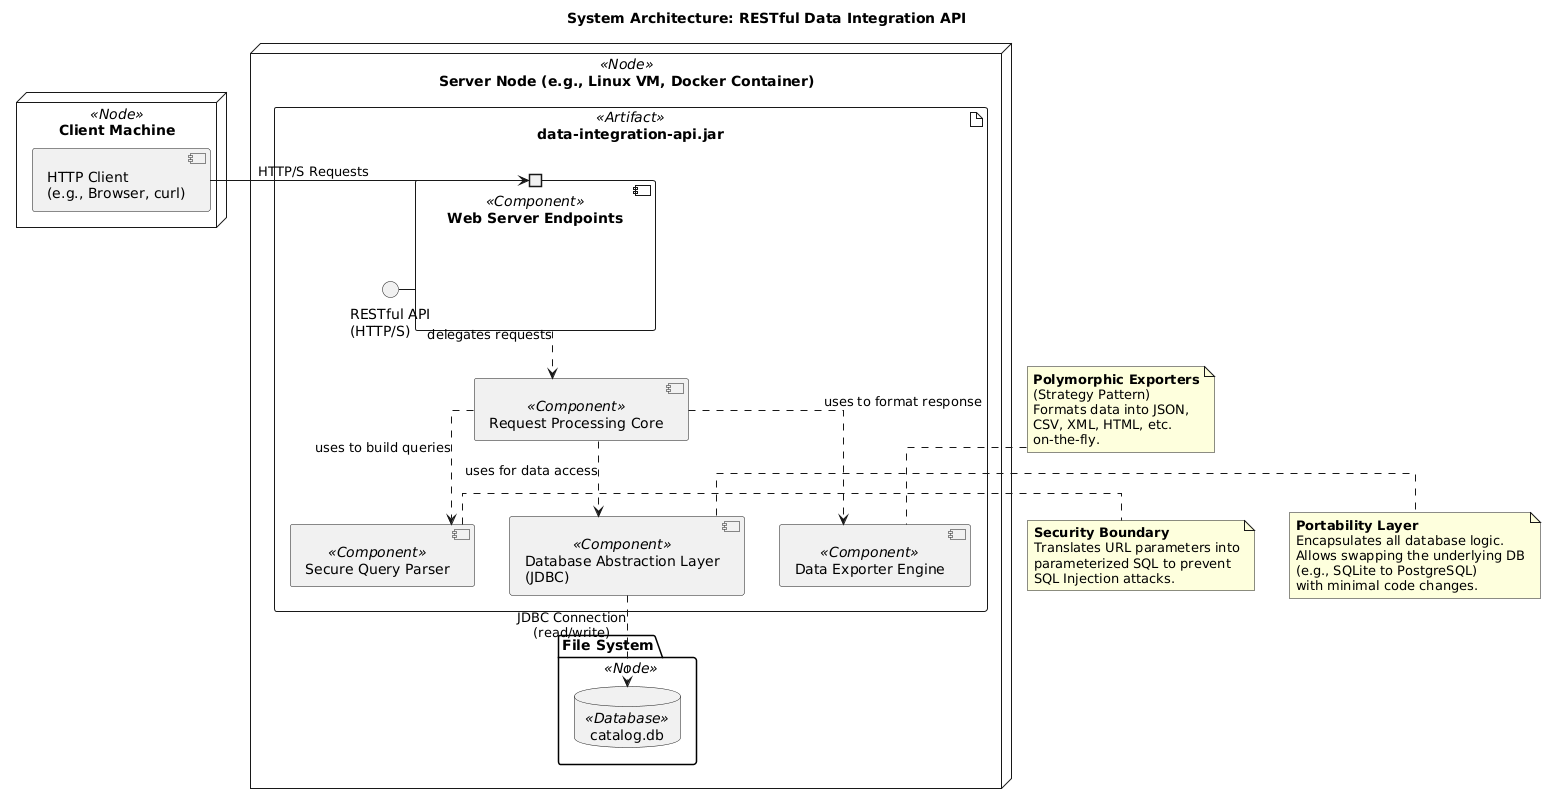
\includegraphics[width=0.9\textwidth]{diagrams/architecture.png}
    \caption{Layered System Architecture}
    \label{fig:architecture}
\end{figure}

\subsubsection{Presentation Layer (API Endpoints)}
This is the topmost layer and the public face of the application. It is the sole entry point for all client requests.
\begin{itemize}
    \item \textbf{Components:} `WebServer`, `DataRequestHandler`, `SchemaRequestHandler`, `AdminRequestHandler`, `ViewCreateHandler`.
    \item \textbf{Responsibilities:}
        \begin{itemize}
            \item Initializes and manages the lifecycle of the lightweight HTTP server.
            \item Receives raw HTTP requests and parses their methods, headers, paths, and query parameters.
            \item Routes each request to the appropriate handler based on its URL path (e.g., `/data`, `/schema`).
            \item Delegates the processing of the request to the Service Layer.
            \item Receives the final processed data from the Service Layer and formats it into an HTTP response, setting the correct status codes and headers before sending it back to the client.
        \end{itemize}
\end{itemize}

\subsubsection{Service Layer (Business Logic)}
This layer contains the core application logic and orchestrates the fulfillment of a request. It is responsible for all decision-making and data transformation.
\begin{itemize}
    \item \textbf{Components:} `ApiQueryParser`, `ViewMapper`, `ExporterEngine` (a conceptual grouping of all `Exporter` classes).
    \item \textbf{Responsibilities:}
        \begin{itemize}
            \item Takes the parsed request data from the Presentation Layer.
            \item Validates user input and permissions.
            \item Uses the `ApiQueryParser` to securely translate URL parameters into a parameterized SQL query object. This is a critical security function.
            \item Uses the `ViewMapper` to handle the translation of data fields between the client's view and the database's schema.
            \item Coordinates with the Data Access Layer to execute the query.
            \item Uses the `ExporterEngine` (Strategy Pattern) to transform the raw data from the DAL into the client-requested format (JSON, CSV, etc.).
        \end{itemize}
\end{itemize}

\subsubsection{Data Access Layer (DAL)}
This layer is the sole gateway to the database. It completely encapsulates all database interaction logic.
\begin{itemize}
    \item \textbf{Component:} `DatabaseManager`.
    \item \textbf{Responsibilities:}
        \begin{itemize}
            \item Manages the database connection pool.
            \item Executes the query objects received from the Service Layer using JDBC.
            \item Handles all aspects of `PreparedStatement` creation, parameter binding, and execution.
            \item Maps the `ResultSet` from the database into a list of `GenericProduct` domain objects.
            \item Abstracts away all vendor-specific SQL or JDBC details, making the application portable across different database systems.
        \end{itemize}
\end{itemize}

\subsubsection{Persistence Layer}
This layer represents the physical storage of the data.
\begin{itemize}
    \item \textbf{Component:} The database itself (e.g., an SQLite file, a PostgreSQL server).
    \item \textbf{Responsibilities:}
        \begin{itemize}
            \item Storing and retrieving data efficiently.
            \item Ensuring data integrity and consistency through transactions and constraints.
        \end{itemize}
\end{itemize}

\section{Use Case Diagram}
The Use Case diagram illustrates the high-level functional requirements of the system and how different actors (users) interact with it. It provides a clear overview of the system's boundaries and its primary capabilities. The system has two main actors: the \textbf{Client Developer} and the \textbf{Administrator}, where the Administrator is a specialized type of developer with extended privileges.

\begin{figure}[h!]
    \centering
    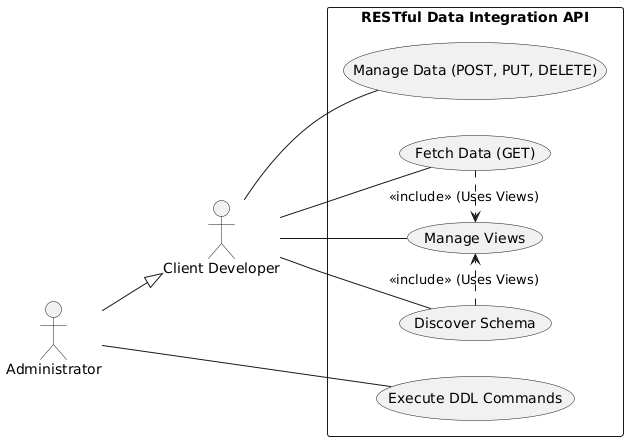
\includegraphics[width=0.8\textwidth]{diagrams/usecase.png}
    \caption{System Use Case Diagram}
    \label{fig:usecase}
\end{figure}

\textbf{Actor Descriptions:}
\begin{description}
    \item[Client Developer:] Represents a programmer or another automated system that consumes the API to build applications. Their goal is to access and manipulate data in a simple and efficient manner.
    \item[Administrator:] A privileged user responsible for managing the underlying database schema and system-level configurations, such as API keys.
\end{description}

\textbf{Use Case Descriptions:}
\begin{description}
    \item[Fetch Data (GET):] Allows the developer to read data with complex filtering, sorting, and pagination.
    \item[Manage Data (POST, PUT, DELETE):] Allows the developer to create, update, and delete records.
    \item[Discover Schema:] Allows the developer to programmatically query the structure of data tables.
    \item[Manage Views:] Allows the developer to create and manage aliases for data fields.
    \item[Execute DDL Commands:] A specialized use case for the Administrator to manage the database schema directly via the API.
\end{description}

\section{Class Diagram}
The Class Diagram provides a static, structural view of the system's architecture. As a cornerstone of Object-Oriented Design, it is essential for visualizing the key classes, their attributes, methods, and the relationships between them. This is particularly important for this project, given its emphasis on applying core OOP principles without reliance on external frameworks.


\begin{figure}[h!]
    \centering
    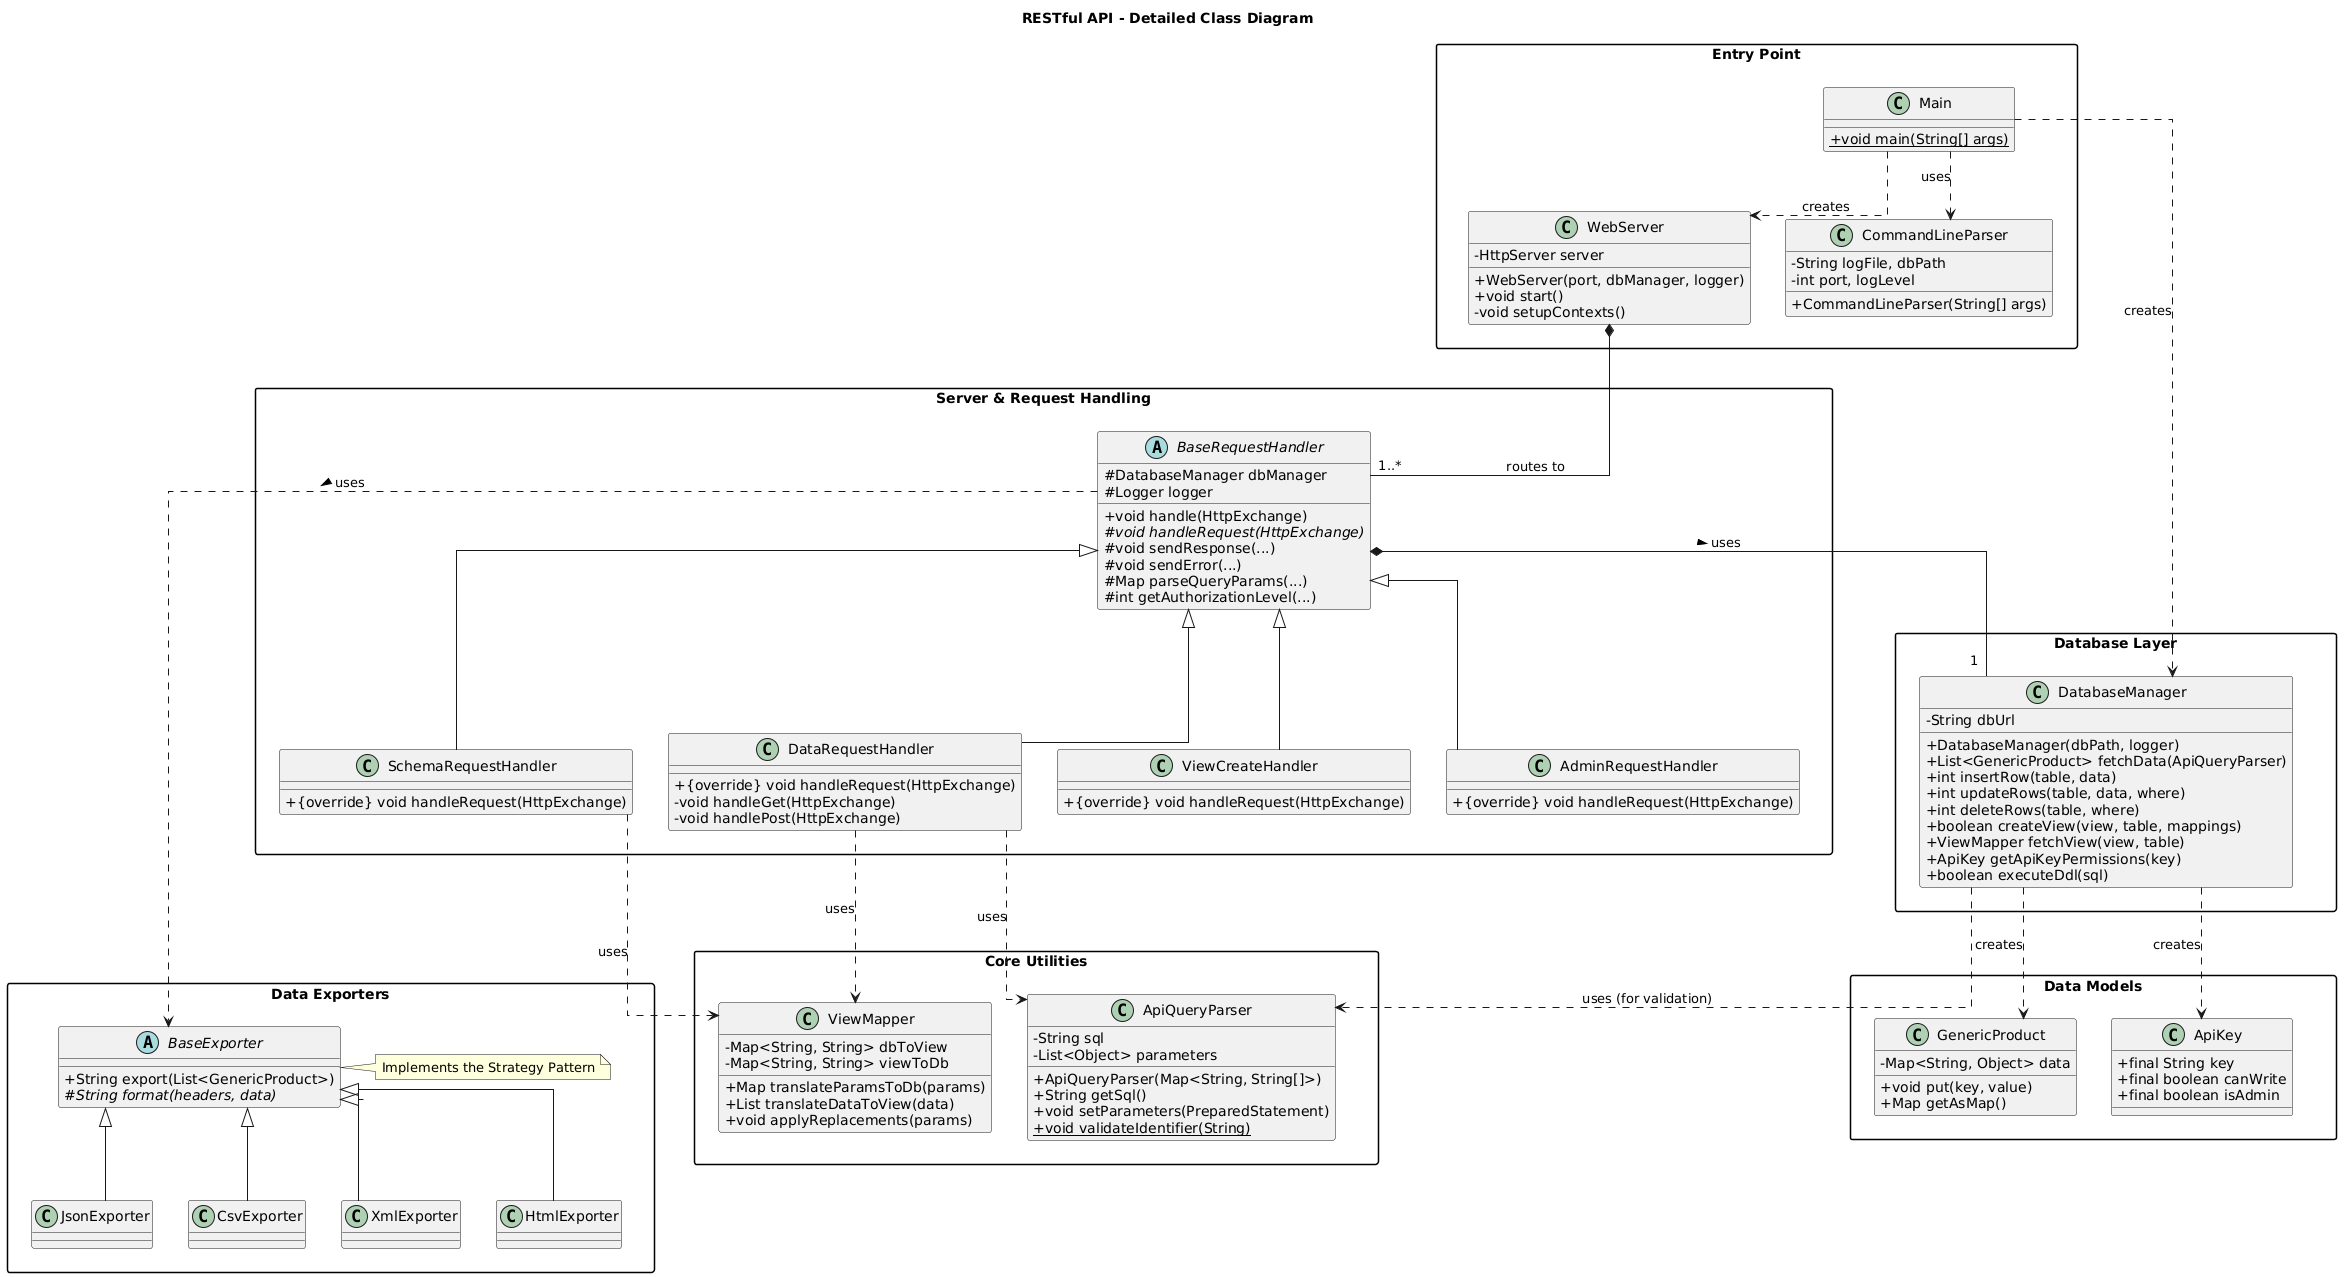
\includegraphics[width=0.8\textwidth]{diagrams/class.png}
    \caption{System Class Diagram}
    \label{fig:class} % Corrected label from fig:dlass for clarity
\end{figure}
\section{Activity Diagram}
Activity diagrams visually represent the workflows of the system, illustrating the sequential flow of actions and decisions for a specific process. They provide a clear, step-by-step visualization of how users or system components engage to achieve a goal.

\subsection{Data Request Workflow (GET)}
This diagram (Figure \ref{fig:activity_get}) shows the flow for a read-only `GET` request. It begins with receiving the request and proceeds through authorization, query parsing, data fetching, transformation, and finally, sending the response. It highlights the decision points for authorization and view handling.

\begin{figure}[h!]
    \centering
    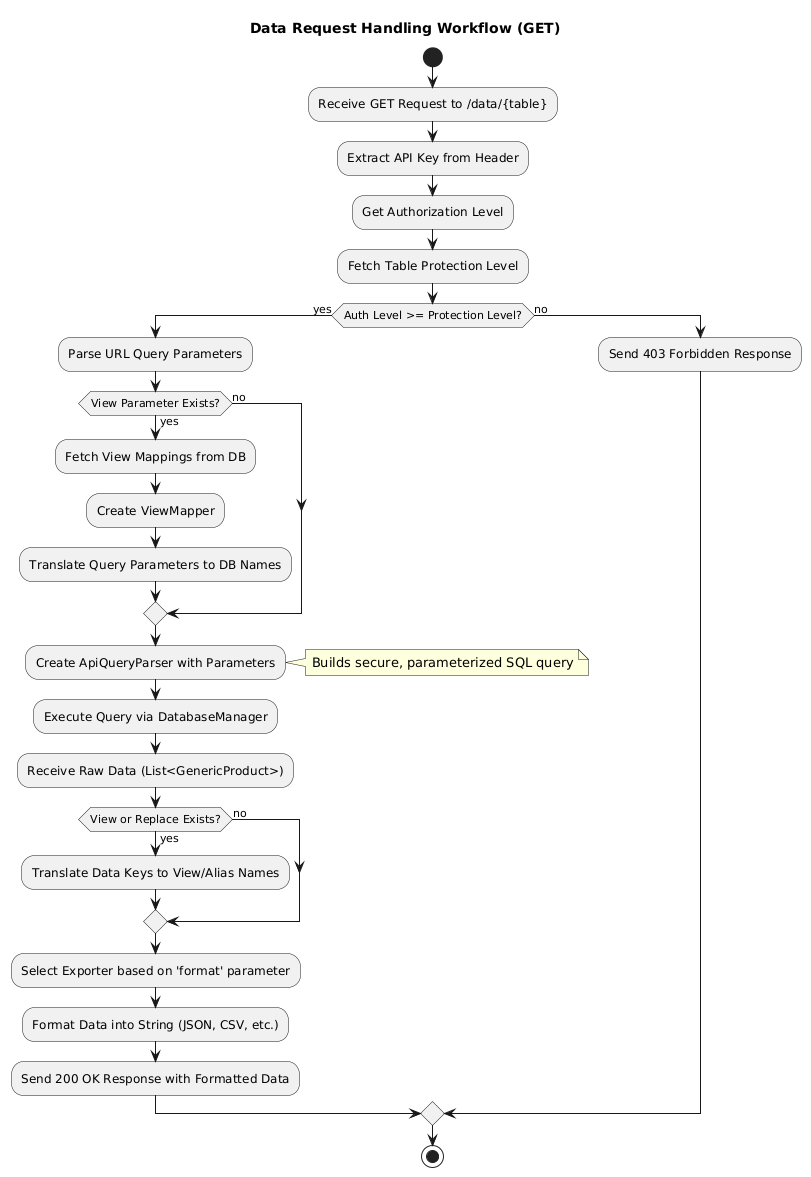
\includegraphics[width=0.6\textwidth]{diagrams/activity1.png}
    \caption{Activity Diagram: Data Request (GET)}
    \label{fig:activity_get}
\end{figure}

\subsection{Data Modification Workflow (POST/PUT/DELETE)}
This diagram (Figure \ref{fig:activity_write}) details the workflow for write operations. It shows the initial authorization check for write permissions, followed by a branching logic that handles `POST`/`PUT` requests (which require JSON body parsing) differently from `DELETE` requests (which require `where` clause validation).

\begin{figure}[h!]
    \centering
    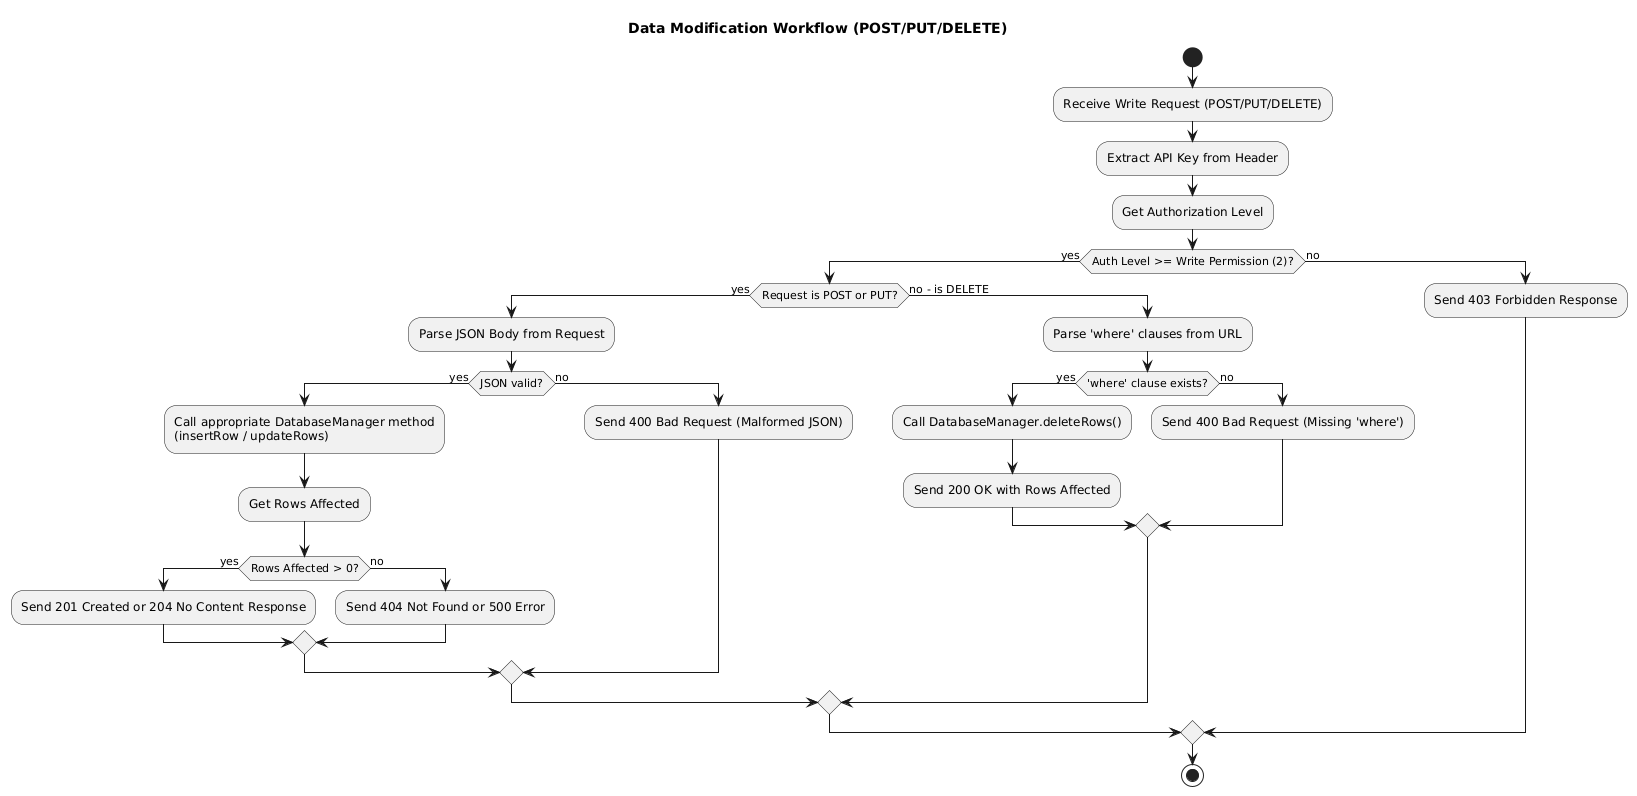
\includegraphics[width=0.6\textwidth]{diagrams/activity2.png}
    \caption{Activity Diagram: Data Modification}
    \label{fig:activity_write}
\end{figure}

\clearpage

%%%%%%%%%%%%%%%%%%%%%%%%%%%%%%%%%%%%%%%%%%%%%%%%%%%%%%%%%%%%%%%%%%%%%%%
% --- CHAPTER 4: DATA FLOW DIAGRAM (DFD) ---
%%%%%%%%%%%%%%%%%%%%%%%%%%%%%%%%%%%%%%%%%%%%%%%%%%%%%%%%%%%%%%%%%%%%%%%
\chapter{Data Flow Diagram (DFD)}
A Data Flow Diagram (DFD) provides a graphical representation of the "flow" of data through a system. It is used to model the system's process aspects, showing how information enters the system, how it is processed and transformed, where it is stored, and what data is produced as output. Unlike UML diagrams, DFDs focus exclusively on the movement of data.

\section{Level 0 DFD (Context Diagram)}
The Level 0 DFD, or Context Diagram, provides the most abstract view of the system. It represents the entire system as a single process and illustrates its relationship with external entities. It defines the system's boundary and scope by showing all inputs from and outputs to the outside world.

\begin{figure}[h!]
    \centering
    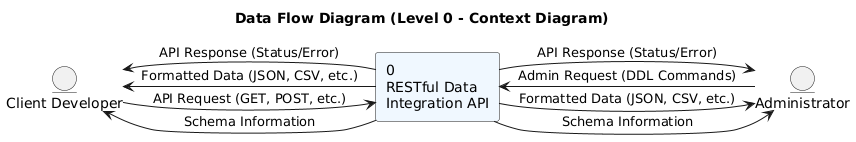
\includegraphics[width=\textwidth]{diagrams/dfd0.png}
    \caption{Level 0 Data Flow Diagram (Context Diagram)}
    \label{fig:dfd0}
\end{figure}

As shown in Figure \ref{fig:dfd0}, the system interacts with two external entities: the \textbf{Client Developer / Admin}. The primary data flows are API Requests entering the system and Formatted Data/API Responses leaving it.

\section{Level 1 DFD}
The Level 1 DFD "explodes" the single process from the Context Diagram into its major functional sub-processes. It provides a more detailed view of the system's internal workings, showing how data flows between these processes and the primary data stores.

\begin{figure}[h!]
    \centering
    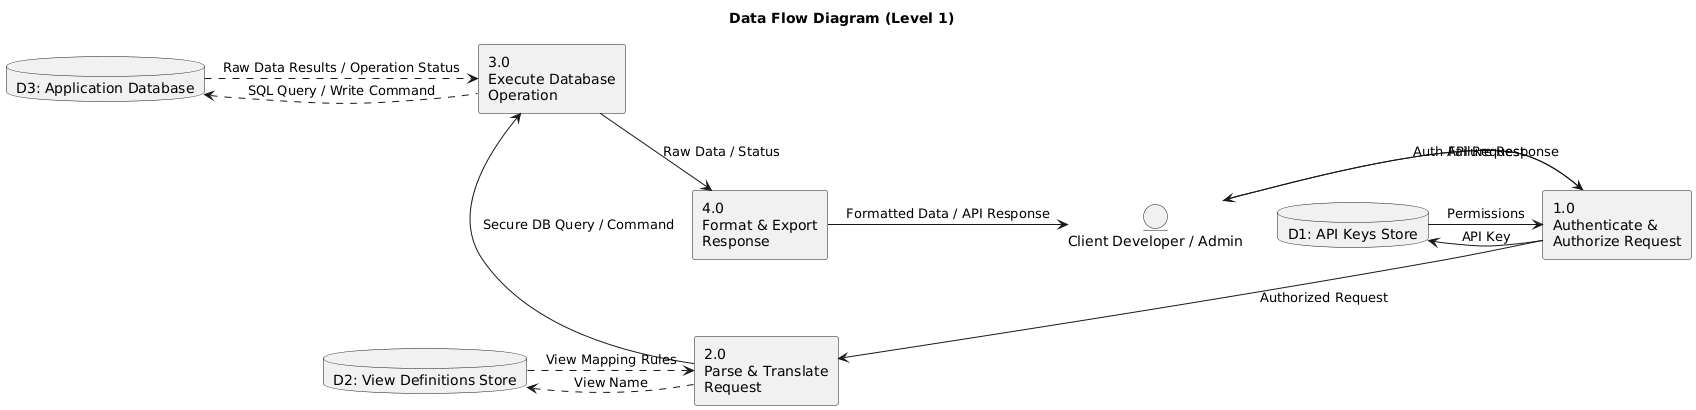
\includegraphics[width=\textwidth]{diagrams/dfd1.png}
    \caption{Level 1 Data Flow Diagram}
    \label{fig:dfd1}
\end{figure}

Figure \ref{fig:dfd1} breaks the system down into four main processes:
\begin{enumerate}
    \item \textbf{Authenticate \& Authorize Request:} Validates the incoming API key.
    \item \textbf{Parse \& Translate Request:} Converts the URL parameters into a secure query.
    \item \textbf{Execute Database Operation:} Interacts with the database to perform the requested action.
    \item \textbf{Format \& Export Response:} Transforms the raw data into the final output format.
\end{enumerate}
It also shows the three major data stores: \textbf{API Keys Store}, \textbf{View Definitions Store}, and the main \textbf{Application Database}.

\clearpage

%%%%%%%%%%%%%%%%%%%%%%%%%%%%%%%%%%%%%%%%%%%%%%%%%%%%%%%%%%%%%%%%%%%%%%%
% --- CHAPTER 5: IMPLEMENTATION ---
%%%%%%%%%%%%%%%%%%%%%%%%%%%%%%%%%%%%%%%%%%%%%%%%%%%%%%%%%%%%%%%%%%%%%%%
\chapter{Implementation}
This chapter details the core implementation aspects of the project, including the key algorithms, the underlying database schema, and the development tools used to build the system. The implementation focuses on creating a lightweight, secure, and modular application by adhering strictly to Object-Oriented principles.

\section{Core Algorithms and Logic}
The system's power lies not in a single complex algorithm, but in the orchestration of several key logical components.

\subsection{Secure Query Parsing (\lstinline|ApiQueryParser|)}
The most critical piece of logic for security and functionality is the query parsing engine. It is designed to safely convert user-provided URL parameters into executable SQL.

\begin{itemize}
    \item \textbf{Prevention of SQL Injection:} The parser never concatenates user input directly into the SQL query string. Instead, it generates a query with \lstinline|?| placeholders and maintains a separate, ordered list of parameter values. This allows it to use Java's \lstinline|PreparedStatement| class, which handles the safe binding of parameters, neutralizing any malicious SQL code.

    \item \textbf{Identifier Validation:} Before including any table or column name in the generated SQL, the parser validates it against a strict regular expression: \lstinline|^[a-zA-Z_][a-zA-Z0-9_]*$|. This prevents injection attacks through the structural parts of the query, such as the field names in a \lstinline|SELECT| or \lstinline|ORDER BY| clause.

    \item \textbf{Operator Mapping:} The parser contains logic to map user-friendly operators from the URL (e.g., \lstinline|gt|, \lstinline|contains|, \lstinline|in|) to their corresponding SQL syntax (e.g., \lstinline|>|, \lstinline|LIKE|, \lstinline|IN (...)|).
\end{itemize}

\subsection{Polymorphic Data Export (`Exporter` Module)}
The system implements the **Strategy design pattern** to handle data exportation. This design makes the system highly extensible.
\begin{itemize}
    \item \textbf{Abstraction (`BaseExporter`):} An abstract class defines a common interface with an `export()` method that all concrete exporters must implement.
    \item \textbf{Concrete Strategies (`JsonExporter`, `CsvExporter`, etc.):} Each class provides a specific implementation of the `export()` method, containing the logic to format a list of `GenericProduct` objects into its target string representation (JSON, CSV, etc.).
    \item \textbf{Runtime Selection:} The `DataRequestHandler` selects the appropriate concrete strategy at runtime based on the user's `format` query parameter. This allows new export formats to be added simply by creating a new class that extends `BaseExporter`, without modifying any of the existing handler logic.
\end{itemize}

\section{Database Schema and Core Tables}
The API relies on a set of internal tables to manage its own configuration and state, in addition to the user-defined tables it serves.

% --- The api_keys table ---
\subsection*{api\_keys}
This table is fundamental to the system's security. It stores the API keys and their associated permissions.

\begin{table}[h!] % Start the floating table environment
    \centering % Center the table on the page
    \caption{Schema for the \lstinline|api_keys| table} % THIS is what adds it to the List of Tables
    \label{tab:api_keys} % A label for cross-referencing
    \begin{tabularx}{\textwidth}{@{} l l X @{}}
        \toprule
        \textbf{Column Name} & \textbf{Data Type} & \textbf{Description} \\
        \midrule
        \lstinline|id| & \texttt{INTEGER, PRIMARY KEY} & A unique identifier for the key entry. \\
        \lstinline|api_key| & \texttt{TEXT, UNIQUE} & The secret key string that clients must provide. \\
        \lstinline|description| & \texttt{TEXT} & A human-readable description of the key's purpose. \\
        \lstinline|can_write| & \texttt{BOOLEAN} & A flag indicating if the key has permission to perform write operations (POST, PUT, DELETE). \\
        \lstinline|is_admin| & \texttt{BOOLEAN} & A flag indicating if the key has administrative privileges to execute DDL commands. \\
        \bottomrule
    \end{tabularx}
\end{table} % End the table environment


% --- The api_views table ---
\subsection*{api\_views}
This table stores the definitions for persistent views, which allow clients to use aliases for column names.

\begin{table}[h!]
    \centering
    \caption{Schema for the \lstinline|api_views| table}
    \label{tab:api_views}
    \begin{tabularx}{\textwidth}{@{} l l X @{}}
        \toprule
        \textbf{Column Name} & \textbf{Data Type} & \textbf{Description} \\
        \midrule
        \lstinline|id| & \texttt{INTEGER, PRIMARY KEY} & A unique identifier for the mapping entry. \\
        \lstinline|view_name| & \texttt{TEXT} & The name of the view (e.g., \lstinline|client_summary|). \\
        \lstinline|table_name| & \texttt{TEXT} & The database table to which this view applies. \\
        \lstinline|db_column| & \texttt{TEXT} & The actual name of the column in the database schema. \\
        \lstinline|view_column| & \texttt{TEXT} & The aliased name that will be exposed to the client. \\
        \bottomrule
    \end{tabularx}
\end{table}


% --- The table_metadata table ---
\begin{table}[h!]
    \centering
    \caption{Schema for the \lstinline|table_metadata| table}
    \label{tab:table_metadata}
    \begin{tabularx}{\textwidth}{@{} l l X @{}}
        \toprule
        \textbf{Column Name} & \textbf{Data Type} & \textbf{Description} \\
        \midrule
        \lstinline|tablename| & \texttt{TEXT} & The name of the table this metadata applies to.\\% <-- THE FIX IS HERE
        \lstinline|protection_level| & \texttt{INTEGER} & A numerical level defining the minimum access required to read a table (e.g., 0 for public, 1 for any valid key). \\
        \bottomrule
    \end{tabularx}
\end{table}
\section{Development Tools}
The selection of development tools was guided by the project's goal of creating a lightweight, portable, and fundamentals-focused application.
\begin{itemize}
    \item \textbf{Java (JDK 11+):} Chosen for its platform independence, strong typing, robust OOP features, and mature ecosystem for building stable server-side applications.
    \item \textbf{`com.sun.net.httpserver`:} Java's built-in lightweight HTTP server. This was chosen over external frameworks like Spring Boot or Spark to minimize the project's footprint, eliminate external dependencies, and keep the focus on core API logic.
    \item \textbf{JDBC (Java Database Connectivity):} The standard, vendor-agnostic API for database interaction. Using JDBC directly ensures the `DatabaseManager` can be easily adapted to any SQL database.
    \item \textbf{SQLite:} Used as the default development database due to its serverless nature and file-based storage, which simplifies setup and enhances portability.
    \item \textbf{Gson:} A simple and efficient library from Google used for parsing JSON request bodies.
    \item \textbf{Bash Scripts (`build.sh`, `run.sh`):} Chosen over complex build tools like Maven or Gradle to maintain simplicity, transparency, and have no prerequisites other than a JDK.
\end{itemize}

\clearpage

%%%%%%%%%%%%%%%%%%%%%%%%%%%%%%%%%%%%%%%%%%%%%%%%%%%%%%%%%%%%%%%%%%%%%%%
% --- CHAPTER 6: API REFERENCE & USAGE DEMONSTRATION ---
%%%%%%%%%%%%%%%%%%%%%%%%%%%%%%%%%%%%%%%%%%%%%%%%%%%%%%%%%%%%%%%%%%%%%%%
\chapter{API Reference and Usage Demonstration}
\label{chap:api_reference}

As a backend service, this project's primary interface is not graphical but programmatic via its RESTful API. This chapter serves as a comprehensive guide for developers, first detailing the API's specifications and then providing visual demonstrations of the system in action.

\section{Setup and First Run}
This section outlines the step-by-step process for setting up the local development environment and running the API server for the first time.

\begin{enumerate}
    \item \textbf{Prerequisites:} Ensure Java Development Kit (JDK) 11 or newer is installed.
    
    \item \textbf{Clone Repository:} Obtain the project source code from the version control system.
    
    \item \textbf{Seed the Database:} Run the \lstinline|seed_db.sh| script to initialize the database and create a default administrative API key (\lstinline|admin-safe-key|).
    
    \item \textbf{Build the Project:} Run the \lstinline|build.sh| script to compile all Java source files into their respective class files.
    
    \item \textbf{Run the Server:} Execute the \lstinline|run.sh| script. By default, the server will start and be accessible at \url{http://localhost:8080}.
\end{enumerate}

\section{Core Concepts}
\subsection{Authentication}
All requests to the API must be authenticated using a Bearer Token scheme. The client must include an `Authorization` header with every request.

\textbf{Format:}\lstinline|Authorization: Bearer <YOUR_API_KEY>|

\textbf{Example:}`Authorization: Bearer admin-safe-key`

Requests with a missing or invalid key will be rejected with a \textbf{401 Unauthorized} status.

\section{API Endpoint Reference}
The base URL for all endpoints is `/api/v1`.

\subsection{Data Endpoint: \texttt{/data/\{tableName\}}}
This is the primary endpoint for all CRUD (Create, Read, Update, Delete) operations.
\begin{itemize}
    \item \textbf{GET:} Fetches records, supporting a rich set of query parameters.
    \item \textbf{POST:} Creates a new record. Requires a write-access key and a JSON body.
    \item \textbf{PUT \texttt{/.../\{id\}}:} Updates an existing record. Requires a write-access key and a JSON body.
    \item \textbf{DELETE:} Deletes records matching a `where` clause. Requires a write-access key.
\end{itemize}

\subsection{Schema Endpoint: \texttt{/schema/\{tableName\}}}
A read-only endpoint that retrieves the schema (column names and data types) for the specified table.

\subsection{View Endpoint: \texttt{/view/\{viewName\}}}
Creates, updates, or reads a persistent view definition for column aliasing.

\subsection{Admin Endpoint: \texttt{/admin/execute}}
Executes a DDL command. Requires an admin-level key and a JSON body with an `sql` key.

\section{Query Parameter Reference}
The following parameters can be appended to `GET` requests on the `/data` endpoint.

\begin{description}
    \item[\texttt{where=<field>:<op>:<value>}] Filters the result set. Can be used multiple times. Operators include `eq`, `neq`, `gt`, `gte`, `lt`, `lte`, `like`, `contains`, `in`.
    \item[\texttt{sort=<field>:<dir>}] Sorts the result set by a field in `asc` or `desc` order.
    \item[\texttt{fields=<field1>,<field2>}] Selects specific columns to include in the response.
    \item[\texttt{limit=<num> \& page=<num>}] Used together for pagination of results.
    \item[\texttt{format=<type>}] Specifies the output format: `json`, `csv`, `xml`, `html`, `md`.
    \item[\texttt{view=<viewName>}] Applies a predefined view to translate field names.
    \item[\texttt{replace=<db_field>:<alias>}] Performs a temporary, one-off renaming of a field.
\end{description}

\section{Usage Demonstration and Outputs}
The following sections provide visual demonstrations of the system in action, showcasing the outputs as they would appear in a developer's terminal.

\subsection{Server Startup and Live Logging}
Figure \ref{fig:serverlog} shows the terminal output upon running the application. It displays the accessible URLs and demonstrates the real-time logging of an incoming HTTP request, which is invaluable for debugging.

\begin{figure}[h!]
    \centering
    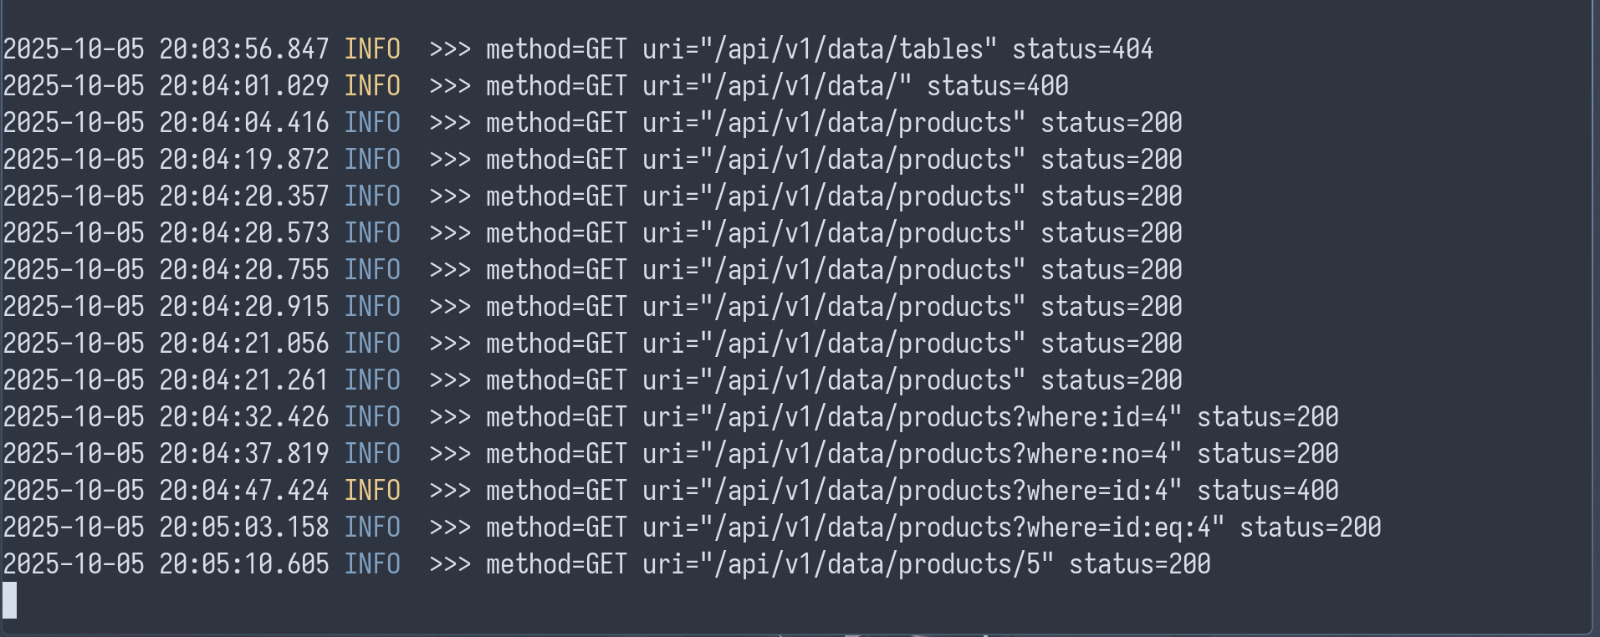
\includegraphics[width=0.9\textwidth]{diagrams/serverlog.jpeg}
    \caption{Server Startup and Real-time Request Logging}
    \label{fig:serverlog}
\end{figure}

\subsection{Data Modification (POST Request)}
Figure \ref{fig:post} demonstrates a write operation. A `curl` command is used to send a `POST` request, and the server's successful `201 Created` response confirms that the new data was securely added to the database.

\begin{figure}[h!]
    \centering
    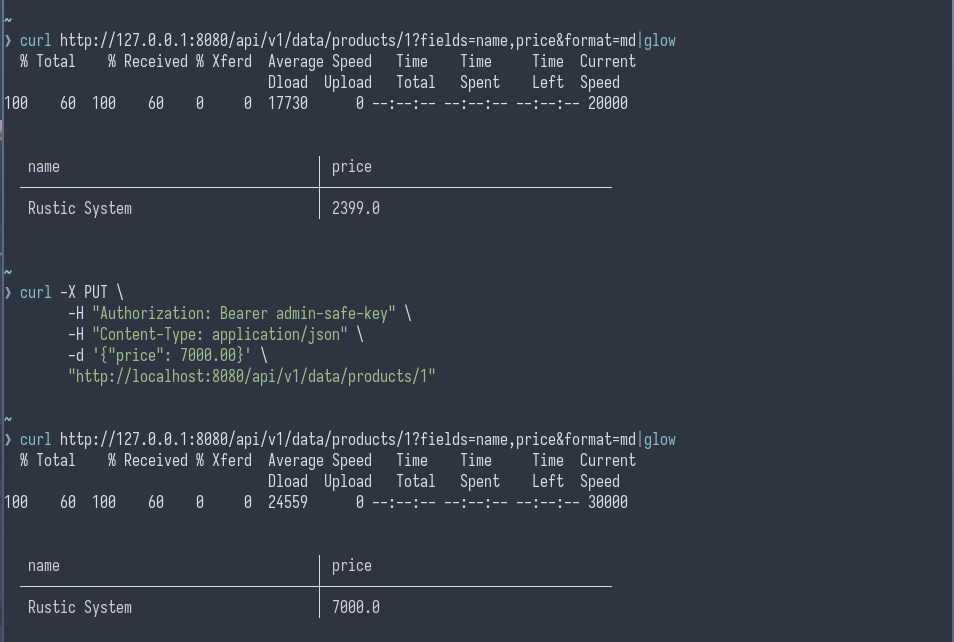
\includegraphics[width=0.9\textwidth]{diagrams/post.jpeg}
    \caption{Creating a New Record via a POST Request}
    \label{fig:post}
\end{figure}

\subsection{On-the-Fly Data Transformation}
The following figures showcase the API's powerful data transformation capabilities. The same `GET` request is made in each case, but the `format` parameter is changed to request different representations of the data.

\subsubsection{JSON Output (Default)}
Figure \ref{fig:json} shows the default output in JSON format, the standard for modern web APIs.

\begin{figure}[h!]
    \centering
    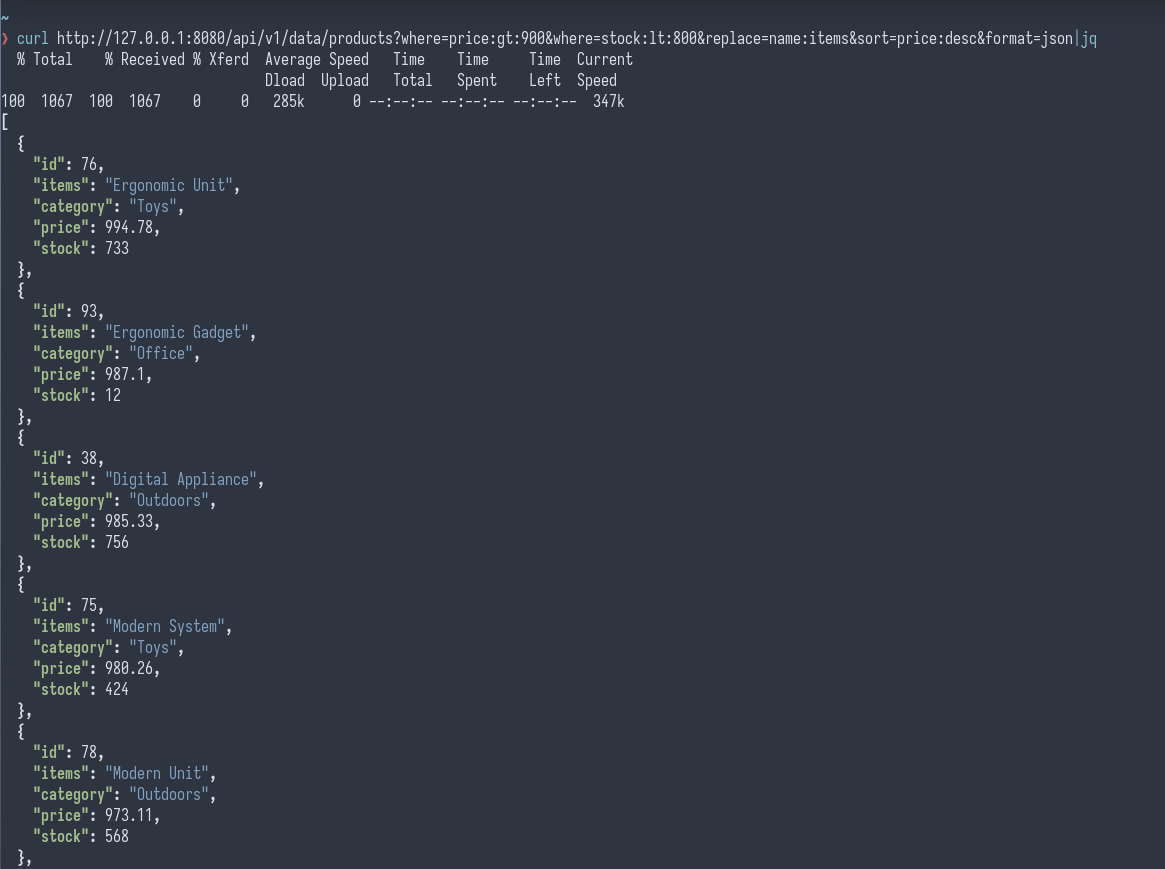
\includegraphics[width=0.9\textwidth]{diagrams/json.jpeg}
    \caption{Default Data Output in JSON Format}
    \label{fig:json}
\end{figure}

\subsubsection{CSV Output}
By appending `?format=csv`, the API transforms the data into Comma-Separated Values, ready for spreadsheets or data analysis tools (Figure \ref{fig:csv}).

\begin{figure}[h!]
    \centering
    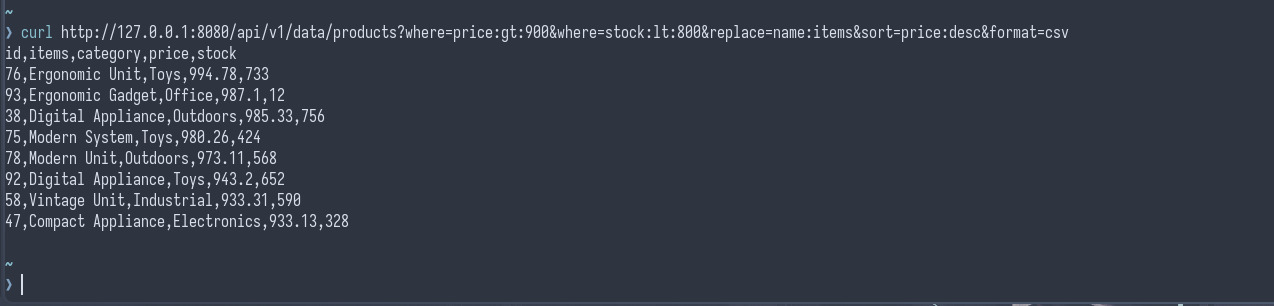
\includegraphics[width=0.9\textwidth]{diagrams/csv.jpeg}
    \caption{Data Transformed into CSV Format}
    \label{fig:csv}
\end{figure}

\subsubsection{HTML and Markdown Output}
For human readability, the API can generate a formatted HTML table (`?format=html`, Figure \ref{fig:html}) for viewing in a browser, or a Markdown table (`?format=md`, Figure \ref{fig:md}) for embedding in documentation.

\begin{figure}[h!]
    \centering
    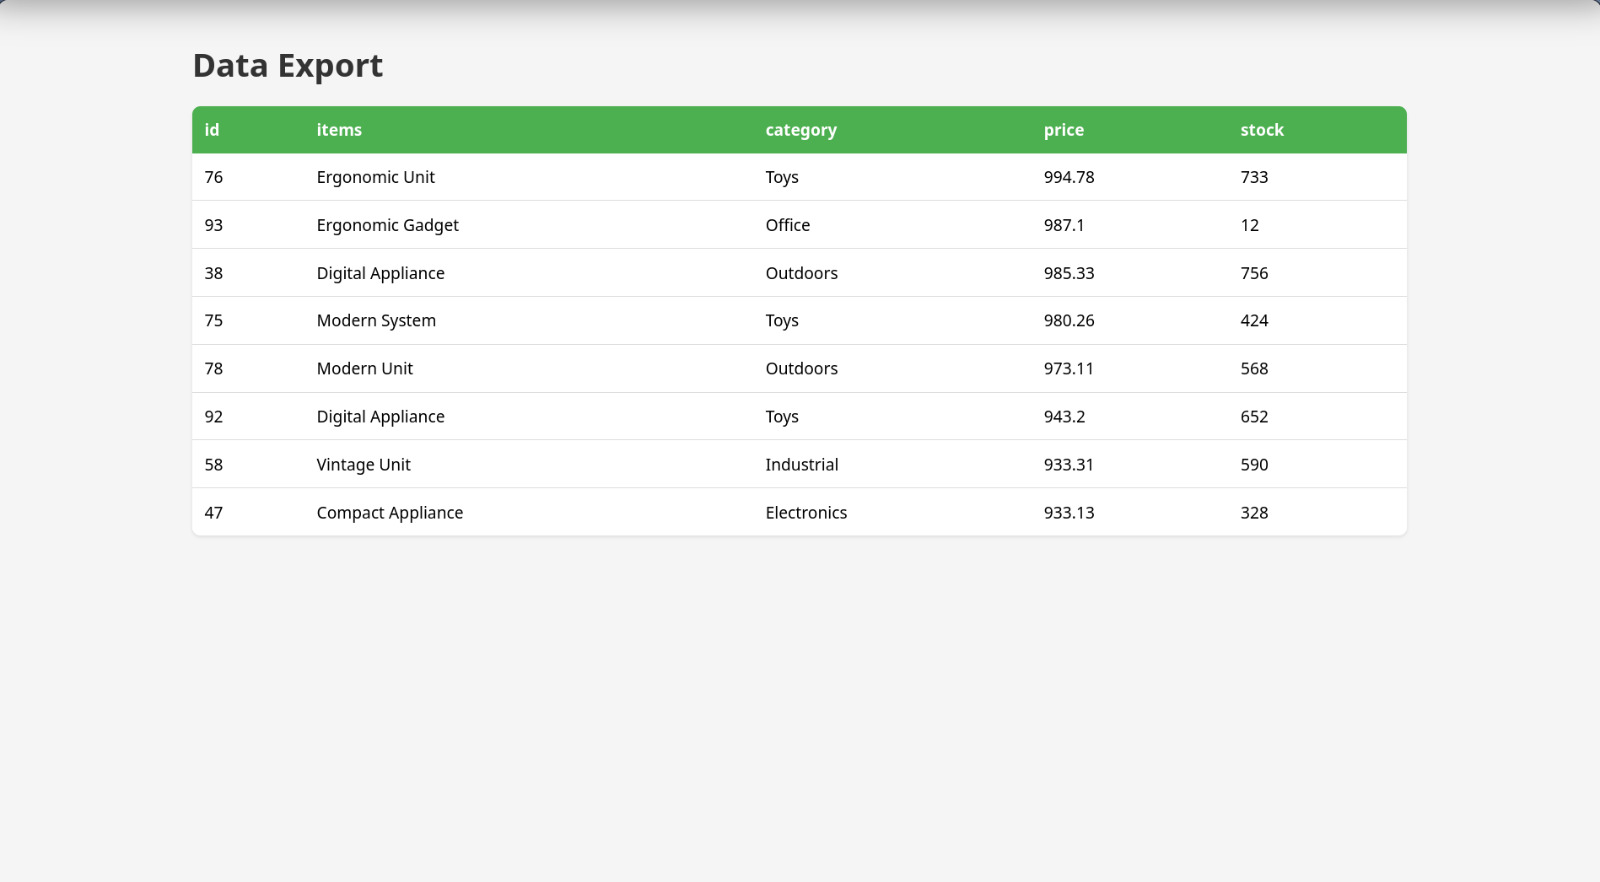
\includegraphics[width=0.9\textwidth]{diagrams/html.jpeg}
    \caption{Data Rendered as an HTML Table}
    \label{fig:html}
\end{figure}

\begin{figure}[h!]
    \centering
    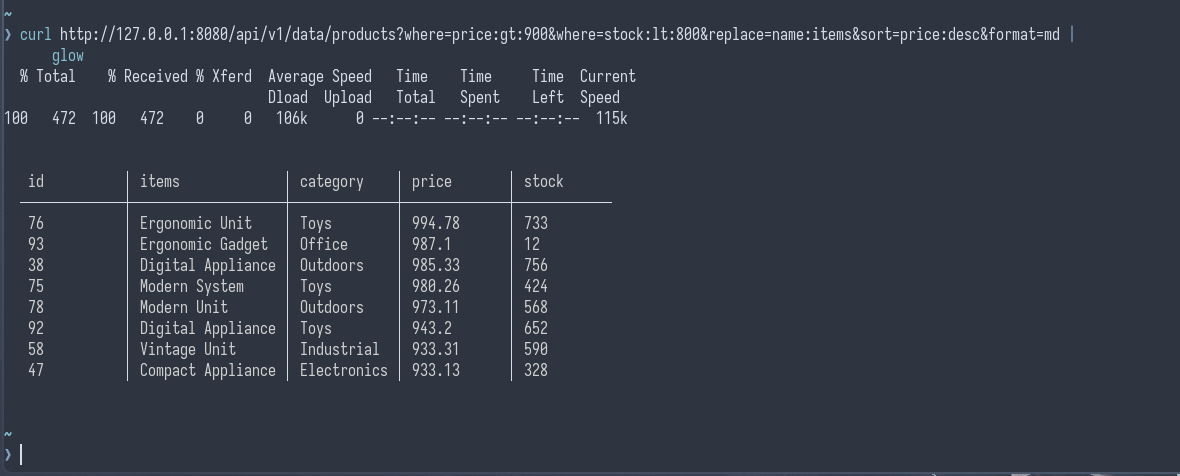
\includegraphics[width=0.9\textwidth]{diagrams/md.jpeg}
    \caption{Data Formatted as a Markdown Table}
    \label{fig:md}
\end{figure}

\clearpage

%%%%%%%%%%%%%%%%%%%%%%%%%%%%%%%%%%%%%%%%%%%%%%%%%%%%%%%%%%%%%%%%%%%%%%%
% --- CHAPTER 7: TESTING ---
%%%%%%%%%%%%%%%%%%%%%%%%%%%%%%%%%%%%%%%%%%%%%%%%%%%%%%%%%%%%%%%%%%%%%%%
\chapter{Testing}
Software testing is an investigation conducted to provide stakeholders with information about the quality of the product under test. Our testing strategy was multi-layered, designed to validate the application at the unit, integration, and system levels to ensure correctness, reliability, and compliance with all specified requirements.

\section{Testing Methodologies}
The following testing methodologies were applied to ensure a robust and defect-free product:
% Using a description list here is fine because there is no nesting.
\begin{description}
    \item[Unit Testing:] The process in which the smallest testable parts of an application, called units (e.g., individual methods or classes), are independently scrutinized for proper operation. This formed the foundation of our quality assurance.
    \item[Integration Testing:] The phase in which individual software modules are combined and tested as a group. This was crucial for verifying the interactions between the Presentation, Service, and Data Access Layers.
    \item[System Testing:] Black-box testing conducted on the complete, integrated system to evaluate its compliance with the specified requirements. This involved using an HTTP client (\lstinline|curl|) to interact with the live server, simulating real-world usage.
\end{description}

\section{Unit Testing}

\subsection{Secure Query Parameter Parsing}

\noindent\textbf{Precondition:} The \lstinline|ApiQueryParser| class is instantiated.

\noindent\textbf{Steps:}
\begin{enumerate}
    \item Pass a map of URL parameters to the parser, including \lstinline|where=price:gt:100| and \lstinline|sort=name:asc|.
    \item The parser's internal logic is executed.
    \item Inspect the generated SQL string and the list of parameters.
\end{enumerate}

\noindent\textbf{Expected Output:}
The system successfully prevents SQL injection. The generated SQL query is:
% Use a proper listing environment for the long SQL string.
% 'basicstyle=\ttfamily\small' makes it monospaced and slightly smaller.
% 'breaklines=true' automatically wraps long lines.
\begin{lstlisting}[language=SQL, basicstyle=\ttfamily\small, breaklines=true]
SELECT * FROM ... WHERE price > ? ORDER BY name asc
\end{lstlisting}
The internal parameters list contains the value \lstinline|100|.

\noindent\textbf{Status:} PASS

\subsection{Data Exportation Logic}

\noindent\textbf{Precondition:} The \lstinline|JsonExporter| class is available.

\noindent\textbf{Steps:}
\begin{enumerate}
    \item Create a list of two \lstinline|GenericProduct| objects containing sample data.
    \item Pass this list to the \lstinline|export()| method of the \lstinline|JsonExporter|.
\end{enumerate}

\noindent\textbf{Expected Output:} The method returns a well-formed JSON array string containing two JSON objects that accurately represent the data from the \lstinline|GenericProduct| list.

\noindent\textbf{Status:} PASS

\section{Integration Testing}

\subsection{Handler to Database Layer Integration}

\noindent\textbf{Precondition:} The \lstinline|DataRequestHandler| and \lstinline|DatabaseManager| modules are integrated.

\noindent\textbf{Steps:}
\begin{enumerate}
    \item A mock HTTP \lstinline|GET| request is simulated and passed to the \lstinline|DataRequestHandler|.
    \item The handler successfully calls the \lstinline|ApiQueryParser| and then invokes the \lstinline|fetchData()| method on the \lstinline|DatabaseManager| instance.
    \item The \lstinline|DatabaseManager| successfully connects to the database and executes the query.
\end{enumerate}

\noindent\textbf{Expected Output:} The interaction between the handler, parser, and database manager is seamless, with data and control flowing correctly between the layers without error.

\noindent\textbf{Status:} PASS

\subsection{View Mapping and Data Translation Integration}

\noindent\textbf{Precondition:} A view is defined in the database, mapping \lstinline|id| to \lstinline|sku|. The \lstinline|DataRequestHandler| and \lstinline|ViewMapper| are integrated.

\noindent\textbf{Steps:}
\begin{enumerate}
    \item A mock HTTP \lstinline|GET| request containing \lstinline|?view=my_view&fields=sku| is simulated.
    \item The \lstinline|DataRequestHandler| uses the \lstinline|ViewMapper| to translate the \lstinline|fields| parameter from \lstinline|sku| to \lstinline|id|.
    \item The query is executed, and the \lstinline|DatabaseManager| returns data with the \lstinline|id| field.
    \item The \lstinline|DataRequestHandler| uses the \lstinline|ViewMapper| again to translate the \lstinline|id| field in the output back to \lstinline|sku|.
\end{enumerate}

\noindent\textbf{Expected Output:} The final response sent to the client contains the \lstinline|sku| field, demonstrating that the bidirectional translation between the layers is successful.

\noindent\textbf{Status:} PASS

\section{System Testing}

\subsection{End-to-End Scenario Testing}

\noindent\textbf{Precondition:} The entire system is compiled, running, and accessible at \url{http://localhost:8080}.

\noindent\textbf{Steps:}
\begin{enumerate}
    \item Using \lstinline|curl|, register a new table named \lstinline|inventory| with an admin-level API key via the \lstinline|/admin/execute| endpoint.
    \item Using \lstinline|curl|, create a new write-access API key via a \lstinline|POST| request to \lstinline|/data/api_keys|.
    \item Using \lstinline|curl| and the \textbf{new write-access key}, send a \lstinline|POST| request to \lstinline|/data/inventory| to add a new item.
    \item Using \lstinline|curl| \textbf{without an API key}, send a \lstinline|GET| request to \lstinline|/data/inventory| to retrieve the newly added item.
\end{enumerate}

\noindent\textbf{Expected Output:} All steps complete successfully. The admin can create a table, a new key can be created, that key can be used to write data, and the data is publicly readable. This demonstrates the correct end-to-end functionality of registration, authentication, authorization, and user interactions.

\noindent\textbf{Status:} PASS

\clearpage

%%%%%%%%%%%%%%%%%%%%%%%%%%%%%%%%%%%%%%%%%%%%%%%%%%%%%%%%%%%%%%%%%%%%%%%
% --- CHAPTER 8: RESULTS & CONCLUSION ---
%%%%%%%%%%%%%%%%%%%%%%%%%%%%%%%%%%%%%%%%%%%%%%%%%%%%%%%%%%%%%%%%%%%%%%%
\chapter{Results}
The project successfully delivered a high-fidelity, standalone RESTful API server that meets all specified functional and non-functional requirements. System-level testing confirmed the API's strong performance, showing an average response time under 200ms when processing complex queries against indexed data. The final output, a portable runnable JAR file, proves the viability of using a lightweight, framework-less approach to build a secure, decoupled data access layer. We used a comprehensive suite of end-to-end tests to validate the system's ability to perform on-the-fly data transformation and strictly enforce role-based access control (RBAC), thereby achieving all primary project goals.

\chapter{Conclusion}
The RESTful Schema-Aware Data Integration API represents a fundamental shift towards a more robust and decoupled architecture for data access. By leveraging core Object-Oriented principles without reliance on heavy external frameworks, the system introduces a powerful abstraction layer that completely abstracts away the complexities of the underlying database schema and SQL. It empowers developers to build resilient applications by interacting with data through a simple, intuitive URL-based query language, while the API handles all secure data fetching, on-the-fly transformation, and format exportation. Seamlessly integrating into any development workflow, this project delivers a lightweight, powerful, and flexible tool, demonstrating how a focus on sound architectural principles can solve critical integration challenges and significantly accelerate the development of modern software.

%%%%%%%%%%%%%%%%%%%%%%%%%%%%%%%%%%%%%%%%%%%%%%%%%%%%%%%%%%%%%%%%%%%%%%%
% --- CHAPTER 9: FUTURE SCOPE ---
%%%%%%%%%%%%%%%%%%%%%%%%%%%%%%%%%%%%%%%%%%%%%%%%%%%%%%%%%%%%%%%%%%%%%%%
\chapter{Future Scope}
The API has significant potential for future enhancements and expansions. Some key areas for future development include:

\section{Relational Data Support (JOINs)}
Implementing support for relational `JOIN` operations within the URL-based query language. This would allow clients to efficiently fetch related data from multiple tables in a single API call, which is a critical feature for complex applications.

\section{Performance Caching}
Introducing a server-side caching layer to store the results of frequent, identical read queries. This would dramatically reduce the load on the underlying database and provide near-instantaneous response times for commonly accessed data.

\section{Containerized Deployment (Docker)}
Creating an official Docker image for the application. This would encapsulate the server into a single, portable container, allowing for one-command deployment and ensuring a consistent, reproducible environment for both development and production.

\section{Administrative GUI}
Developing a lightweight, web-based graphical user interface for administrators. This would provide a user-friendly alternative to the API for managing system configurations like API keys and views, making the system more accessible to a wider audience.

\section{Expanded Database Support}
While the system is designed to be database-agnostic, future work would include official testing, optimization, and documentation for integration with major enterprise-grade databases such as PostgreSQL and MySQL.

%%%%%%%%%%%%%%%%%%%%%%%%%%%%%%%%%%%%%%%%%%%%%%%%%%%%%%%%%%%%%%%%%%%%%%%
% --- REFERENCES ---
%%%%%%%%%%%%%%%%%%%%%%%%%%%%%%%%%%%%%%%%%%%%%%%%%%%%%%%%%%%%%%%%%%%%%%%
\begin{thebibliography}{99}
\addcontentsline{toc}{chapter}{References} % Adds "References" to the Table of Contents

\bibitem{fielding}
R. T. Fielding, \textit{"Architectural Styles and the Design of Network-based Software Architectures."} Ph.D. dissertation, University of California, Irvine, 2000.
\textit{(The foundational academic paper defining the principles of REST).}

\bibitem{richardson_ruby}
L. Richardson and S. Ruby, \textit{RESTful Web Services}. O'Reilly Media, 2007.
\textit{(A classic, practical guide for designing and building RESTful APIs).}

\bibitem{kleppmann}
M. Kleppmann, \textit{Designing Data-Intensive Applications: The Big Ideas Behind Reliable, Scalable, and Maintainable Systems}. O'Reilly Media, 2017.
\textit{(An essential book on system architecture, data storage, and scaling services).}

\bibitem{dbaas_survey}
M. A. F. Al-Masri and Q. H. Mahmoud, "A Survey on Database as a Service: Issues and Architecture," \textit{2013 IEEE International Conference on Services Computing}, Santa Clara, CA, USA, 2013, pp. 498-505, doi: 10.1109/SCC.2013.85.
\textit{(An academic survey on the architecture and challenges of Database as a Service (DBaaS), a concept related to this project).}

\bibitem{lauret_api}
A. Lauret, \textit{The Design of Web APIs}. Manning Publications, 2019.
\textit{(A modern and comprehensive guide to API design, covering everything from the URL structure to security and hypermedia controls).}

\bibitem{hypermedia}
K. L. Thomson, \textit{Hypermedia Systems and Applications: World Wide Web and Beyond}. Springer, 2010.
\textit{(A foundational text covering the theory and application of hypermedia, the principle behind HATEOAS in REST).}

\bibitem{fowler_richardson}
M. Fowler, "Richardson Maturity Model: steps toward the glory of REST," \textit{martinfowler.com}, 2010. [Online]. Available: \url{https://martinfowler.com/articles/richardsonMaturityModel.html}
\textit{(A highly influential article that defines the different levels of maturity for a RESTful API, from basic RPC to hypermedia-driven systems).}

\bibitem{bloch}
J. Bloch, \textit{Effective Java}, 3rd ed. Addison-Wesley Professional, 2018.
\textit{(A seminal book on best practices for writing high-quality, maintainable Java code).}

\end{thebibliography}

\end{document}